\RequirePackage{fix-cm}
\documentclass[smallextended,natbib]{svjour3}

\usepackage{graphicx}
\usepackage{hyperref}

\usepackage{todonotes}
\newcommand{\todoI}[1]{\todo[author=isak,color=green]{#1}}
\newcommand{\todoP}[1]{\todo[author=panos,color=gray]{#1}}
\newcommand{\todoJ}[1]{\todo[author=jon,color=red]{#1}}
\newcommand{\todoA}[1]{\todo[author=aris,color=green]{#1}}

\usepackage[utf8]{inputenc}

\usepackage{amssymb} 
\usepackage[ruled,noline,linesnumbered,noend]{algorithm2e}
\usepackage{amsmath} 
\usepackage{blindtext}
\usepackage{graphicx}
\usepackage{natbib}

\usepackage{booktabs}
\usepackage{pgfplotstable}

\usepackage{subcaption} 
\captionsetup{compatibility=false}
\usepackage{caption}

\usepackage{tikz}
\usetikzlibrary{trees}

\journalname{Data Mining and Knowledge Discovery}

\title{Actionable Shapelet Tweaking for Time Series Classification}
\author{...}
\date{March 2018}

\begin{document}

\maketitle

TODOs
\begin{enumerate}
\item  motivation and examples from application areas where actionable shapelets are useful.

\item  ensemble version: Optimal solution. If shapelets are matching it can be hard.NP hard (possibly). 

\item improve the greedy version by pruning paths.

\item handle contradicting tweaks.

\item [DONE] Simple version: decision tree. Look at TP paths and find the one with the smallest cost; convert each feature decision.

\item [DONE] ensemble version: Greedy solution. Look at each TN tree. Find the smallest cost path. Apply the changes to the time series example. Try the next tree; until the ensemble changes the decision. 

\end{enumerate}

\section{Motivation}
Recently, the generalized random shapelet forest (gRSF) \citep{KarlssonPB16} has been proposed for univariate and multi-variate time series classification. The main idea is to build a set of decision trees, where each feature corresponds to a \emph{shapelet}. The decision condition on an internal node is the presence or absence of a shapelet in a test time series example.

Despite its competitive performance in terms of classification accuracy on a large collection time series datasets, gRSF is an opaque classification model. It is hence not feasible to come up with any reasoning behind the predictions that could possible be helpful to domain experts and practitioners.

Our main objective is to describe a theoretical framework for extracting interpretable and actionable uni-variate and multi-variate shapelet features for the task of time series classification. Let $\mathcal{T}$ be a multi-dimensional time series and $f(\cdot)$ denote the classification function. Consider the binary classification problem, where $\mathcal{T}$ may belong to either the positive class (+1) or negative class (-1). Consider a test example $\mathcal{T}$ for which $f(\mathcal{T}) = -1$. Our task is to identify the minimum number of changes to be applied to $\mathcal{T}$, i.e., in terms of a cost function $c(\cdot)$, such that $f(\mathcal{T}) = 1$.

\section{Our story in short}
Given a time series example and an opaque classifier (e.g., the gRSF), we want to suggest the smallest number of changes so that the classifier changes the classification from True Negative to True Positive. 

The smallest number of changes in our case corresponds to the smallest number of shapelets that should be tweaked.  There are two types of tweaks:
\begin{itemize}
\item if a shepelet exists in the time series (i.e., occurs within distance $\leq \theta$), we want to increase the distance of its best match to $> \theta$.
\item if a shapelet does not exist in the time series (i.e., its distance is $> \theta$), we want to decrease the distance of its best match to $\theta$.
\end{itemize}

\smallskip
\noindent
\textbf{Algorithm 1: input (time series T), output (tweaked time series $\hat{T}$)}
\begin{enumerate}
    \item identify the trees in the gRSF that classify T as negative.
    \item for each negative tree t, try to change the prediction, by exploring the positive paths in t.
    \item for each positive path in t, identify the shapelets involved in the path, and invert the matching condition in T, by tweaking the segment of the best match of each shapelet.
    \item if the tweaked version of T does not change the ensemble prediction, ignore it; otherwise keep track of it
    \item loop across all negative trees and find the path with the lowest cost
\end{enumerate}

Different distance measures can be used. We will explore two: Euclidean and DTW. Hence the key subproblem: given two time series T and S, and a distance threshold $\theta$, what is is the minimum number of changes in T so that the distance to S is changes from $\leq \theta$ to $> \theta$ or (ii) vice-versa?

\smallskip
\noindent
\textbf{Euclidean Distance:} consider each time series as a k-dimensional point.
\begin{itemize}
    \item define the circle around the point of interest, i.e., S, with radius $\theta$.
    \item if $ED(T,S) \leq \theta$, then $T$ falls inside the circle. $\hat{T}$ is then the point on the circle that intersects the line connecting the two points.
\end{itemize}

The simplest case is for a time series of length 2. Let the shapelet be $S=(S_x, S_y)$ and the target time series match $T=(T_x,T_y)$. The set of similar to $S$ time series $T$ within a Euclidean similarity $\theta$ fall within the circle defined as follows:
\begin{equation}
\label{eq:circle}
   (x-T_x)^2+ (y-T_y)^2 = \theta^2 
\end{equation}

In addition, the line formed by the two points, S and T is defined as follows:
\begin{equation}
\label{eq:line}
   y = S_y + \frac{T_y-S_y}{T_x-S_x} (x-S_x)
\end{equation}

Hence, the time series feature tweaking problem for the 2-D case, is simply the solution of the system of Eq. \ref{eq:circle} and \ref{eq:line}.  

\begin{figure}[h]
\centering
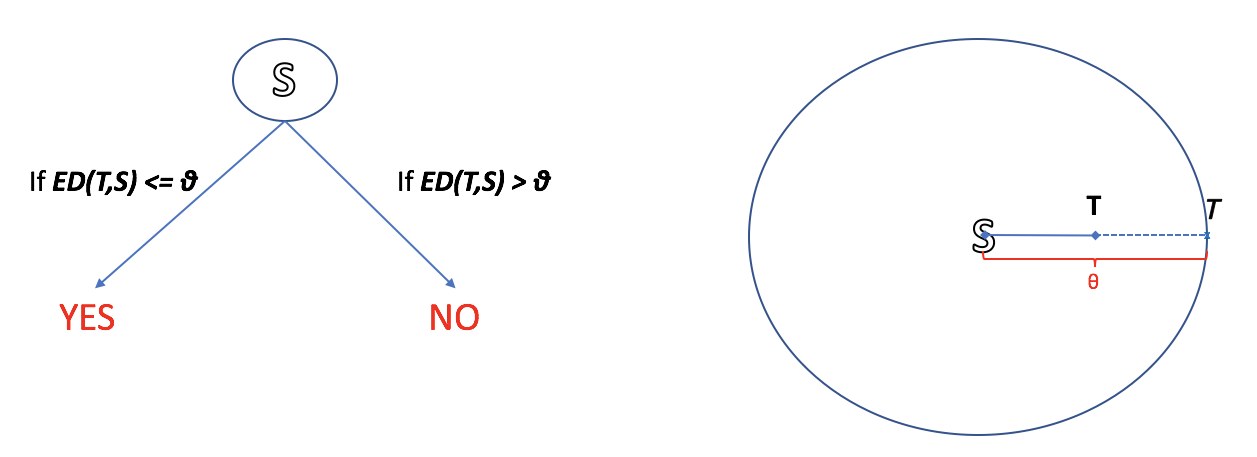
\includegraphics[scale=0.2]{exampleED.png}%
\caption{Example of time series tweaking under the ED.}\label{fig:exampleED}
\end{figure}


\section{Background}
\begin{definition} \textbf{($d$-dimensional time series)} %
A \emph{$d$-dimensional time series} $\mathcal{T} = \{\vec{T_{1}}, \ldots, \vec{T_{d}}\}$ is a sequence of $d$ variables, such that $\vec{T}_k\in \mathbb{R}^m$, $\forall k\in\{1,\dots,d\}$, where $\vec{T_k}=\{T_{k,1},\ldots,T_{k,m}\}$, with $T_{k,j}\in \mathbb{R}$, $\forall j\in\{1,\dots,m\}$. For $d=1$, $\mathcal{T}$ defines a \emph{univariate} time series, denoted simply as $\mathcal{T}=\{T_1,\ldots,T_m\}$ consisting of a sequence of $m$ ordered elements $T_j \in \mathbb{R}$. For $d>1$, $\mathcal{T}$ defines a \emph{multivariate} time series.
\end{definition}

A local segment of a time series is called a \emph{time series subsequence}. A more formal definition is given next.

\begin{definition} \textbf{(time series subsequence)} 
 A \emph{time series sub\-sequence} of the $k^{th}$ dimension of a time series $\mathcal{T}$ is a sequence of $l$ contiguous elements of $\vec{T}_k$, denoted as $\vec{T}_{k}^{s:s+l-1} = \{T_{k,s}, \ldots, T_{k,s+l-1}\}$, where $s$ is the starting position and $l$ is its length. Time series sub\-sequence and shapelet is used interchangeably.
\end{definition}

Time series classification predominantly relies on the chosen distance (similarity) measure to compare and discriminate between instance pairs. The main task is to employ a distance function $dist(\cdot)$ that compares two time series of equal length, and then given a time series subsequence (corresponding to a candidate discriminant shapelet) identify the closest subsequence match in the target time series. Depending on the application domain and the nature of the time series, various distance measures can be used.

\begin{definition} \textbf{(time series sub\-sequence distance)} 
Given a $1$-dimensional time series $\mathcal{S}$ and a $d$-dimensional time series $\mathcal{T}$ of lengths $l$ and $m$, respectively, such that $l \leq m$, the \emph{time series sub\-sequence distance} between $\mathcal{S}$ and the $k^{th}$ dimension of $\mathcal{T}$, is the minimum distance between $\mathcal{S}$ and any sub\-sequence of $\vec{T}_k$ of length $l$, i.e.:
\begin{equation}
  Sdist(\mathcal{S}, \vec{T}_k) = \min_{s=1}^{m-l+1} \{ 
  dist (\mathcal{S}, \vec{T}_k^{s:s+l-1}) \} \ .
\end{equation}
Note that since a $\mathcal{S}$ is $1$-dimensional time series of length equal to the length of each sub\-sequence $\vec{T}_k'^{s:s+l-1}$, dist can be applied directly.
\end{definition}

One possible distance function for $dist(\cdot)$ is the Euclidean distance.
\begin{definition} \textbf{(time series Euclidean distance)} %
Given two time series $\mathcal{T}$ and $\mathcal{T'}$ of equal length $l$, the distance between their corresponding $k^{th}$ dimensions is the length-normalized Euclidean distance between $\vec{T}_k$ and $\vec{T}_k'$, i.e.:
\begin{equation}
 dist(\vec{T}_k,\vec{T}_k') = ED (\vec{T}_k,\vec{T}_k') =  \sqrt{\frac{1}{l} \sum_{i=1}^{l}(T_{k,i}-T_{k,i}')^2} \ .
\end{equation}
 
\end{definition}
Finally, we define the distance between a time series sub\-sequence and a time series.

A collection of $n$ time series $\mathcal{D} = \{\mathcal{T}^{1},\ldots,\mathcal{T}^{n}\}$ defines a \emph{time series dataset}. 

\begin{definition} \textbf{(time series classification function)} %
  Given a dataset $\mathcal{D}$ of $n$ time series and a finite set of
  labels $\mathcal{C}$, a classification function is a mapping
  $f : \mathcal{D} \rightarrow \mathcal{C}$, such that for each
  $\mathcal{T}^{i}\in \mathcal{D}$

\[
f(\mathcal{T}^{i}) = \hat{y}_i\in \mathcal{C} \ ,
  \forall i\in \{1,\dots,n\} \ .
\]
\end{definition}

\subsection{Problem formulation}
Let $\mathcal{R} = \{F_1, \dots, F_k\}$ be a shapelet tree ensemble of $k$ members, where each $F_i$ is a shapelet tree. Consider a time series test example $\mathcal{T}$, and for simplicity let us focus on the univariate case. 

Suppose that the predicted class by $\mathcal{R}$ for $\mathcal{T}$ is $f(\mathcal{T}) = y$, which also equals the actual class of $\mathcal{T}$ and we want to change the time series to flip the prediction to another label $y'$. The objective is to identify \emph{a transformation} $\tau{\mathcal{T}} = \mathcal{T}'$ for which the prediction of $f(\mathcal{T}') = y'$.

\section{Proposed Method}

\subsection{Decision stump}
The simplest problem in our setting is a decision stump. Given a decision node, a shapelet $\mathcal{S}$, a time series $\mathcal{T}$, and a matching threshold $\theta$, we can have two possible settings:
\begin{equation}
f(\mathcal{T}) = 
\begin{cases}
    1,& \text{if } Fdist(\mathcal{S}, \mathcal{T}) \leq \theta\\
    -1,              & \text{otherwise}
\end{cases}
\end{equation}

Or alternatively, 
\begin{equation}
f(\mathcal{T}) = 
\begin{cases}
    1,& \text{if } Fdist(\mathcal{S}, \mathcal{T}) > \theta\\
    -1,              & \text{otherwise}
\end{cases}
\end{equation}

\subsection{Greedy algorithm}

Given an ensemble $\mathcal{R}$ of $k$ shapelet trees\footnote{With unscaled (i.e., not z-normalized) shapelets}, we convert each path from the root node to a leaf node for each tree to a bag of rules per label. Lets denote a rule (decision list) as $DL^j_{c=y}$ (i.e., the $j$:th rule predicting $y$). Each rule consist of a sequence of condition $C_1,\ldots,C_P$ which are represented by the triple $C_p=(\tau, \mathcal{S}, \theta')$. In the condition triplet, $\tau$ is either $\leq$ or $>$, $\mathcal{S}$ is the shapelet used in the comparison and $\theta'$ is the distance threshold. We say that a time series is covered by a condition if $\tau(Sdist(\mathcal{S}, \mathcal{T}), \theta)$ is true and we say that a time series if covered by a rule if all conditions of the rule are true. In the greedy algorithm, we collect all rules resulting in a particular prediction and denote this bag as $DL_{c=y}=[DL^{j}_{c=y},\ldots,DL^{J}_{c=y}]$. For instance, $DL_{c=1}$ contains all rules that predicts a time series as $y=1$ and $DL_{c=5}$ all rules that predicts a time series as $y=5$.

Given a time series $\mathcal{T}$ predicted as some label $y$, and a desired label $y'$ where $y \neq y'$ and a bag of rules predicting $y'$, i.e., $DL_{c=y'}$, the greedy algorithm applies a sequence of transformations $\mathcal{T}' = \Delta(C^p, \mathcal{T})$ for each rule $DL^j_{c=y'}$, starting with applying the first condition $\mathcal{T}'_1 = \Delta(C^1, \mathcal{T})$ to the original time series, and continue to apply all subsequent conditions to the resulting time series, i.e., $\mathcal{T}'_{p+1} = \Delta(C^p, \mathcal{T}'_{p})$.

\begin{figure}
    \centering
    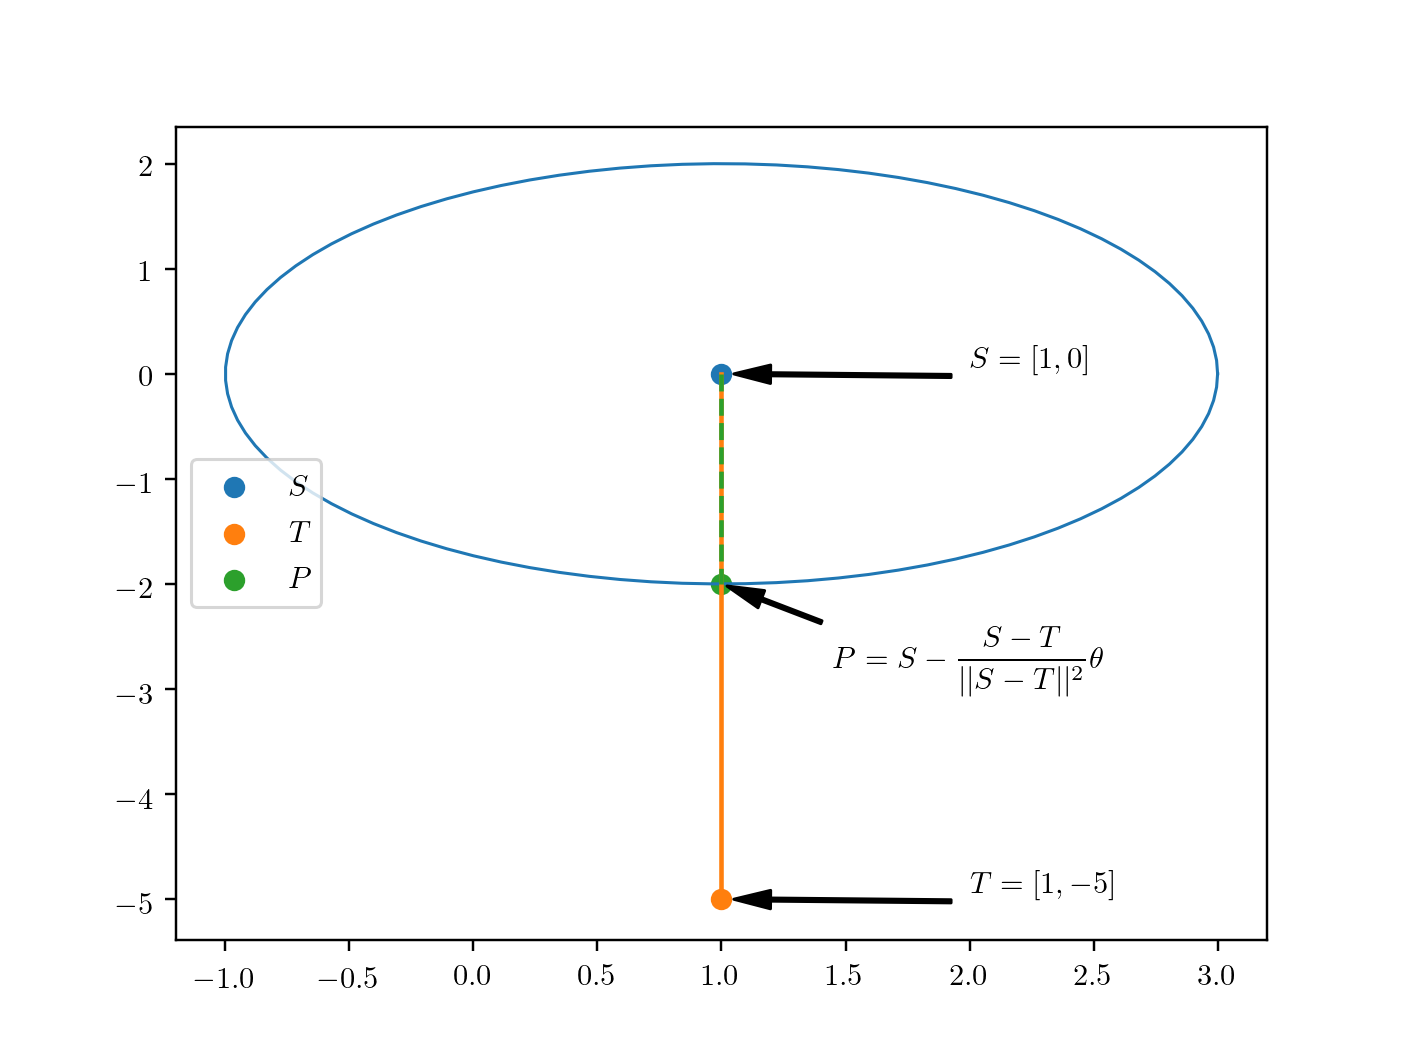
\includegraphics[width=0.7\textwidth]{example.png}
    \caption{Example of moving the point $T$ to the closest point on the circle representing the distance threshold $\theta$, where the distance between $dist(\mathcal{S}, \mathcal{T}) = \theta$}
    \label{fig:move:example}
\end{figure}

A transformation is needed when $\tau(Sdist(\mathcal{S}, \mathcal{T}), \theta)$ is false, i.e., when $\tau$ is $\leq$ and $Sdist(\mathcal{S}, \mathcal{T}) > \theta$ or when $\tau$ is $>$ and $Sdist(\mathcal{S}, \mathcal{T}) \leq \theta$. In the first case i.e.,  when the closest match is larger than the threshold but we want it to be smaller, the transformation is simple: we find the shapelet (starting at $s$ and ending at $e$) with the closest match and apply Eq.\ref{eq:move} (see Fig.~\ref{fig:move:example}) with $\epsilon$ set to a small \emph{negative} constant to move the shapelet slightly closer than $\theta$ and replaces the shapelet in $\mathcal{T}'_{p+1}=\mathcal{T}'^{(s:e)}_{p} = \mathcal{P}$ (abusing notation, this means that the shapelet starting at $s$ and ending at $e$ in $\mathcal{T}$ is replaced by $\mathcal{P}$ and assigned to $\mathcal{T}'$). In the second case, i.e., when the closest match is smaller than the threshold but we want it to be larger, the transformation is slightly more convoluted since there might exist many position where the distance is smaller than $\theta$. In the greedy approach, we simply transform each matching position in order (ignoring that transformations might overlap), according to Eq.~\ref{eq:move} with $\epsilon$ set to a small \emph{positive} constant to move the shapelet slight farther away than $\theta$ and replace the corresponding shapelet with $\mathcal{P}$.

\begin{equation}
 \mathcal{P} = \mathcal{S} - \frac{\mathcal{S} - \mathcal{T}^{(s:e)}}{\lVert \mathcal{S} - \mathcal{T}^{(s:e)} \rVert^2}(\theta+\epsilon)
 \label{eq:move}
\end{equation}

Then, for each rule of the target label $y'$, we transform the time series $\mathcal{T}$ to $\mathcal{T}'_1,\ldots,\mathcal{T}'_J$ and select the time series with the minimum Euclidean distance to the original time series, i.e., $\lVert \mathcal{T} - \mathcal{T}'_j\rVert^2$, and where the transformation is successfully according to the ensemble, i.e., $f(\mathcal{T}'_j) = y'$.  


An example can be seen in Fig.~\ref{fig:greedy:example:1} where a time series representing different insects flying through a audio recording device. The original time series (blue) denotes an insect labeled as $1$ and the red time series denote the same time series after being transformed to an insect labeled as $5$. The gray dashed line represent the closes neighbour to the transformed time series among insects labeled $5$. A similar example is show in Fig.~\ref{fig:greedy:example:2} for the four transformations with lowest transformation cost, i.e., the transformations most similar to the original time series.  

\begin{figure}
    \centering
    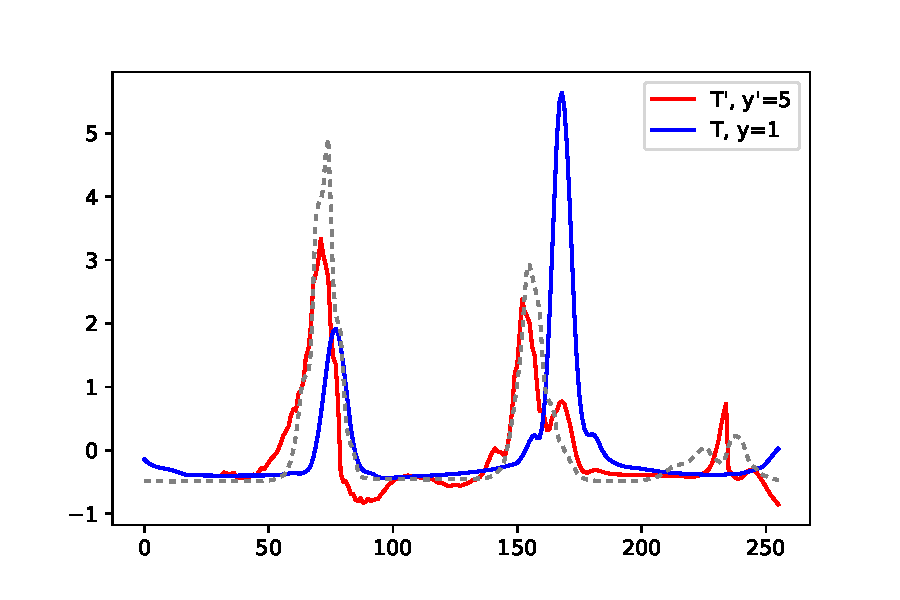
\includegraphics[width=0.7\textwidth]{figure/greedy/example1.pdf}
    \caption{Example of converting the time series $\mathcal{T}$ (blue) with $y=1$ to a transformed time series $\mathcal{T}'$ (red) with label changed to $y'=5$. The gray dotted line denotes the nearest neighbour of $\mathcal{T}$ among the time series labeled as $y'=5$}
    \label{fig:greedy:example:1}
\end{figure}

\begin{figure}
    \centering
    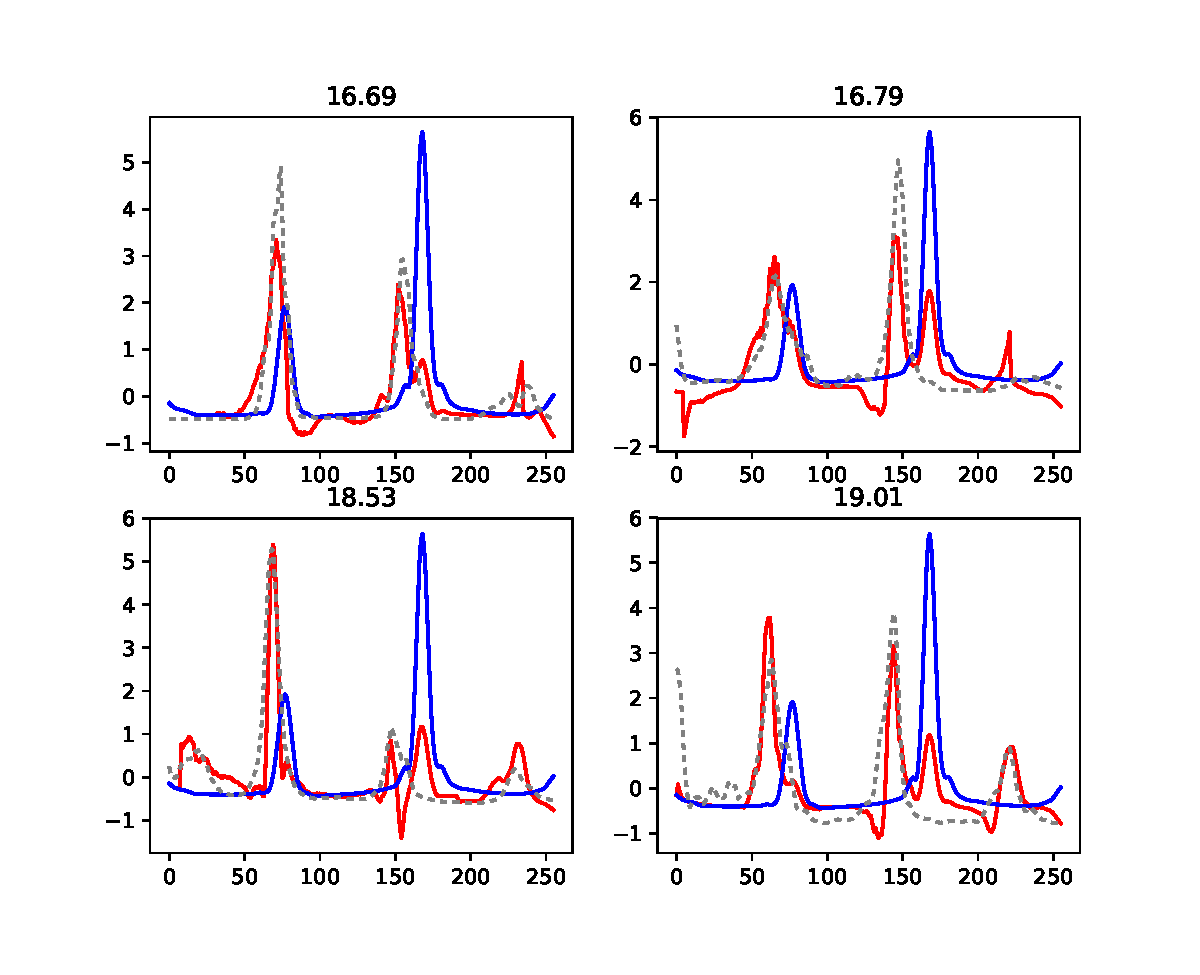
\includegraphics[width=0.8\textwidth]{figure/greedy/example2.pdf}
    \caption{Example of converting the time series $\mathcal{T}$ (blue) with label $y=1$ to a transformed time series $\mathcal{T}'$ (red) for which the label is predicted as $y'=5$, for the four least costly transformations, as measured by the Euclidean distance, i.e., $\lVert \mathcal{T} - \mathcal{T}'\rVert^2$.}
    \label{fig:greedy:example:2}
\end{figure}



\bibliographystyle{spbasic} 
\bibliography{references}


\end{document}
